\section{C-SVM}

\section{The C-Support Vector Machine (C-SVM)}

\mode<presentation>{
\begin{frame} 
    \begin{center} \huge
        \secname
    \end{center}
    \begin{center}
    No longer assuming perfect separability + regularizing SVMs 
    \end{center}
\end{frame}
}

\begin{frame}\frametitle{Classification of non-separable problems}
	\begin{minipage}{12cm}
		\begin{minipage}{6cm}
			\begin{itemize}
				\item  real-world problems are typically non-separable
				\vspace{1mm}
				\item incomplete feature sets \& noise
				\vspace{1mm}
				\item perfect separation of the training set $\leadsto$ overfitting
			\end{itemize}
		\end{minipage}
		\hfill
		\begin{minipage}{4.5cm}
			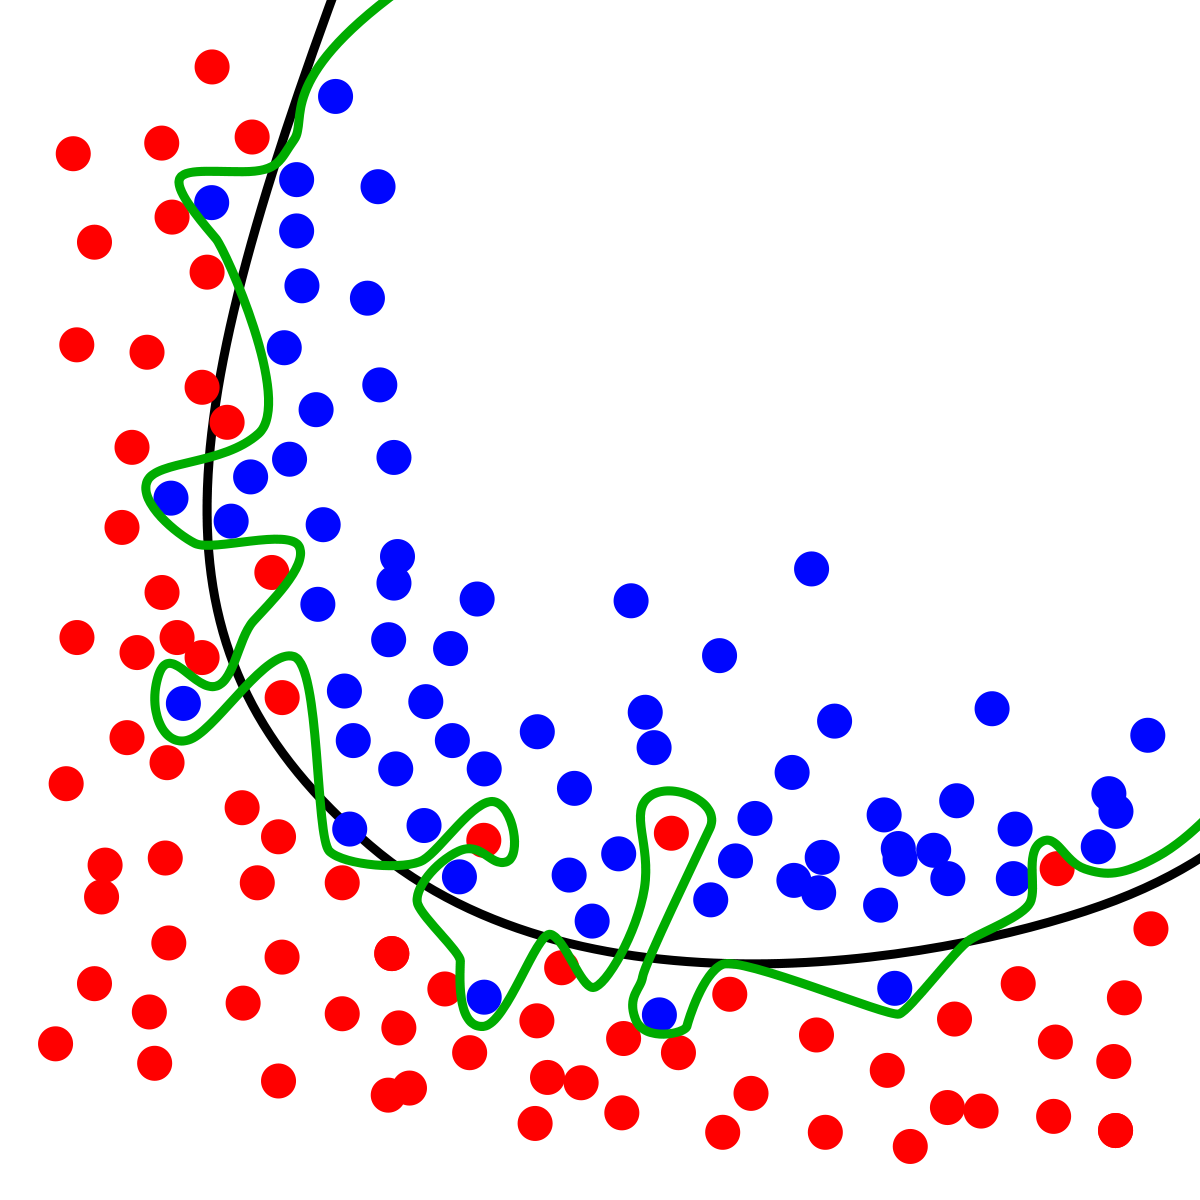
\includegraphics[height=3.5cm]{img/overfitting-classification.png}
		\end{minipage}
	\end{minipage}
	
	\pause

	\begin{block}{consequences}
		$$
			R_{[\vec w]} \quad\leq\quad 
			R_{\emp [\vec w]}^{(p)} \;\;+\;\; C(p,\dvc)
		$$
		\vspace{-3mm}
		\begin{itemize}
			\item finite training error $R_{\emp}^{(p)} \neq 0$ 
			\item trade-off between the minimization of the training error \\
		  		and the capacity of the model class.\\
		  		\slidesonly{Remember weight decay and LASSO regularization?}
		  		
		  		\notesonly{This is similar to the trade-off when regularizing connectionist neurons with weight decay or LASSO regularization. We no longer assume that minimizing the training error is representative of a good solution, particularly in terms of generalizing to unseen data.}
		\end{itemize}
	\end{block}
\end{frame}

\subsection{The primal problem of the C-SVM}

% -----------------------------------------------------------------------------
\begin{frame}\frametitle{\subsecname}
	\begin{block}{} 
	\vspace{-4mm}
	\begin{equation}\label{eq:primal-problem-csvm}
		\begin{array}{ll}
		\frac{1}{2} \|\vec{w}\|^2 
				\visible<2->{{\color{blue} + \frac{C}{p} 
				\sum\limits_{\alpha = 1}^p \varphi_\alpha}}
			\eqexcl \min \;\;\Bigg\{
		& \begin{array}{l}
			\scriptsize{\text{minimize upper bound on VC dimension}} \\
			\visible<2->{\scriptsize{\text{\color{blue}
				+ minimize (approx.) margin error}}}
		\end{array}
		\end{array}
	\end{equation}

	{constraints ($\forall \alpha$):}
	\hfill \only<2>{\scriptsize{{\color{blue}($C$: regularization parameter)}} \normalsize}
	\begin{equation}
		\begin{array}{rll}
			y_T^{(\alpha)} \Big( \vec{w}^\top \vec{x}^{(\alpha)} + b \Big)
				&\geq 1 
				\visible<2->{\color{blue} - \varphi_\alpha}
			& \substack{\text{normalization \& correct classification} \\[1mm]
					\text{of all data points, i.e. ``no slack''}  
					\visible<2->{\color{blue} \text{ for } \varphi_\alpha = 0 } } \\ 
			\visible<2->{\color{blue} \varphi_\alpha & \color{blue} \geq 0 
			& \scriptstyle \color{blue} \text{``margin errors'' for } 
				\varphi_\alpha \neq 0 \text{ ``with slack''}}
		\end{array}
	\end{equation}
	\end{block}
	
	\begin{center}
		\includegraphics<1>[height=3.cm]{img/margin_and_weights}	
		\includegraphics<2>[height=3.cm]{img/margin_errors}	
	\end{center}
	%\begin{itemize}
	%	\itR C: regularization-parameter $\leadsto$ model selection
	%	\itR Why margin error? $\leadsto$ margin necessary for bounding $\dvc$
	%\end{itemize}
	
	\question{How does ${\color{blue}C}$ control complexity?}
	
	\question{How does ${\color{blue}C}$ control complexity?}
	
\end{frame}


% ----------------------------------------------------------------------------
\begin{frame}\frametitle{The dual problem of the C-SVM}

	\begin{itemize}
	\item Objective
		\begin{equation}
			-\frac{1}{2} \sum\limits_{\alpha,\beta = 1}^p \lambda_\alpha
				\lambda_\beta y_T^{(\alpha)} y_T^{(\beta)} 
				\underbrace{ \Big( \vec{x}^{(\alpha)} \Big)^\top 
					\vec{x}^{(\beta)}}_{\text{kernel function}}
				+ \sum\limits_{\alpha = 1}^p \lambda_\alpha 
				\quad \eqexcl \quad \max_{\{\lambda_\alpha\}_{\alpha=1}^p}
		\end{equation}
		
		\notesonly{
		See \sectionref{sec:dualtoprimal} for the derivation. The Lagrangian is the same for SVMs and C-SVMs.
		The difference is in the constraints.
		}
	%\vspace{3mm}
	\item Constraints:
		\begin{equation}
			\sum\limits_{\alpha = 1}^p \lambda_\alpha y_T^{(\alpha)} = 0 \qquad \text{and} \qquad
			0 \leq \underbrace{\lambda_\alpha 
				\;\;{\color{blue}\leq \frac{C}{p}} }_{
				\substack{ \color{blue} \text{difference to} \\
					\color{blue} \text{separable case}}} 
		\end{equation}
	\end{itemize}
	\mode<presentation>{
	\vspace{-5mm}
	\begin{center}
		\includegraphics<2>[height=3.cm]{img/margin_errors}	
	\end{center}
	}
\end{frame}

% -----------------------------------------------------------------------------
\begin{frame} \frametitle{Margin and support vectors}
	\begin{center} 
		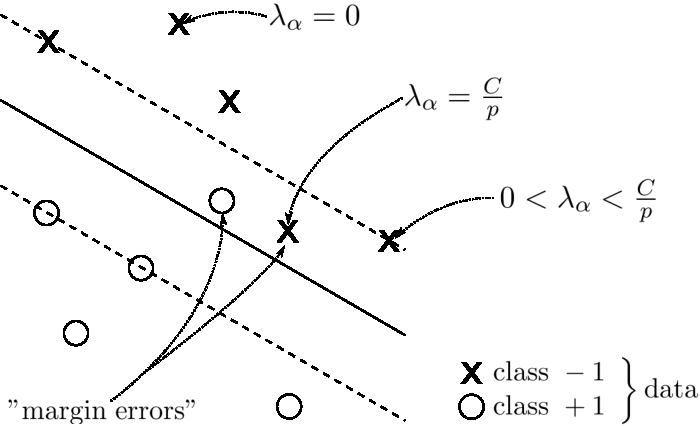
\includegraphics[height=5cm]{img/section2_fig16_v2} 
	\end{center}
	
	\question{Where are the support vectors?}
	
	\pause
	
	\question{Does $C$ influence the number of support vectors?}
	
	
\end{frame}

% -----------------------------------------------------------------------------
\begin{frame}\frametitle{The C-SVM classifier}

SVs do not necessarily lie on the margin anymore. The C-SVM has a ``soft'' margin.

\slidesonly{\vspace{-3mm}}

	\begin{eqnarray*}
		\vec{w} &=& \sum\limits_{\alpha = 1}^p \lambda_\alpha y_T^{(\alpha)}
			\vec{x}^{(\alpha)} \qquad
		\leadsto {\color{red}\lambda_\alpha \neq 0} \text{ only for support vectors }SV\\[2mm]
		\pause
		b &=& \frac{1}{\# SV_<} \sum\limits_{\alpha \in SV_<} \bigg( y_T^{(\alpha)}
			- \sum\limits_{\color{red}\beta \in SV} \lambda_\beta y_T^{(\beta)} 
			\underbrace{ \Big( \vec{x}^{(\beta)} \Big)^{\kern-0.6ex\top} 
				\kern-0.2ex\vec{x}^{(\alpha)}}_{\text{kernel function}}
			\bigg)
	\end{eqnarray*}
	\vspace{2mm}
	$SV_<$: $SV$s with $0 < \lambda_\alpha < \frac{C}{p}$ 
	($SV$s on the margin) 
	
	\pause

	\begin{block}{Classifier}
	\begin{equation*}
		%\hat 
		y(\vec x) = \sign \big( \vec{w}^\top \vec{x} + b \big) 
		= \sign \bigg( \sum\limits_{\alpha \in SV} \lambda_\alpha y_T^{(\alpha)} 
			\underbrace{ \Big( \vec{x}^{(\alpha)} \Big)^{\kern-0.6ex\top} 
				\kern-0.2ex \vec{x}}_{
				\text{kernel function}} + \;b
			\bigg)
	\end{equation*}
	\end{block}
\end{frame}

\begin{frame}
C-SVM demo: \href{https://cs.stanford.edu/people/karpathy/svmjs/demo/}{Link to C-SVM applet}
\end{frame}
